\documentclass[12pt]{scrartcl}
\usepackage{notes_2023}

\begin{document}
	\title{Il gruppo dei quaternioni}
	\maketitle
	
	Si illustra in questo documento il \textbf{gruppo dei quaternioni}, spesso
	e volentieri impiegato in teoria dei gruppi per fornire controesempi. Storicamente
	si definisce tale gruppo, indicato con $Q_8$, come il gruppo formato dai
	quaternioni $\pm 1$, $\pm i$, $\pm j$ e $\pm k$ sotto le usuali regole
	dei moltiplicazione di $\HH$. In particolare, si può definire $Q_8$ mediante
	la seguente presentazione:
	\[ Q_8 = \gen{i, j \mid i^2 = j^2, i^4 = j^4 = e, ij = j^3 i}, \]
	dove $1 := e$, $k := ij$ e $-1 := i^2$. In particolare $-i := i^3$ è l'inverso
	di $i$, $-j := j^3$ quello di $j$ e
	$-k := j^3 i$ quello di $k$. Si osserva che $Q_8$ ha otto elementi, sei di ordine
	$4$ ($\pm i$, $\pm j$ e $\pm k$), uno di ordine $2$ ($-1$)
	e, ovviamente, uno di ordine $1$ ($1$). \medskip
	
	
	Le moltiplicazioni tra $i$, $j$ e $k$ si possono riassumere col seguente
	diagramma:
	\[  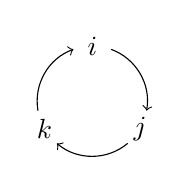
\begin{tikzpicture}[->,scale=.7] % rubato a Diego Monaco -- dispense di Algebra 1, p. 52
		\foreach \a/\t in {90/i,-30/j,210/k}{
			\node (\t) at (\a:1cm) {$\t$};
			\draw (\a-20:1cm)  arc (\a-20:\a-100:1cm);
		} 
		\end{tikzpicture}
	\]
	
	Moltiplicando in senso orario viene restituito il terzo termine, in senso
	antiorario viene restituita la terza potenza del terzo termine rimanente
	(per esempio, $ik=j^3=-j$, si ``aggiunge'' in pratica il segno meno). \medskip

	
	Si possono classificare molto facilmente i sottogruppi di $Q_8$, che sono:
	
	\begin{itemize}
		\item $Q_8$ stesso, di ordine $8$, banalmente normale,
		\item $\gen{i}$, $\gen{j}$ e $\gen{k}$, di ordine $4$, normali perché
			di indice $2$,
		\item $\gen{-1}$ di ordine $2$, normale perché caratteristico (è l'unico sottogruppo
			di ordine $2$ ed è anche il centro $Z(Q_8)$ di $Q_8$),
		\item $\{1\}$, di ordine $1$, banalmente normale.
	\end{itemize}
	
	Pertanto $Q_8$ è un esempio di gruppo non abeliano i cui sottogruppi sono tutti normali
	(e in particolare anche ciclici).
	Inoltre $Q_8$ non può essere decomposto non banalmente in un prodotto semidiretto
	tra i suoi sottogruppi: andrebbero infatti scelti due sottogruppi di ordine $4$, che,
	essendo normali, indurrebbero obbligatoriamente un prodotto diretto tra gruppi ciclici;
	poiché questo prodotto è abeliano, $Q_8$ non può essergli isomorfo.
\end{document}